\section{Project 9 - Image Segmentation}

\subsection{Project Proposal}
There tow parts of project 9. One task is for edge detection: implement the Roberts, Prewitt, Sobel, the Marr-Hildreth and the Canny edge detectors. The test image is \emph{building.tif}. The other task is to implement the Otsu’s method of thresholding segmentation, and compare the results with the global thresholding method using test image \emph{polymersomes.tif}.

\subsection{Preliminaries}
\subsubsection{Edge detection}
The central idea of edge detection is that local changes in intensity can be detected using derivatives. We have the following conclusions which show that first- and second-order derivatives are particularly well suited for this purpose: (1) First-order derivatives generally produce thicker edges in an image. (2) Second-order derivatives have a stronger response to fine details such as thin lines, isolated points, and noise. (3) Second-order derivatives produce a double-edge response at ramp and step transitions in intensity. (4) The sign of the second derivative can be used to determine whether a transition into an edge is from light to dark or dark to light.

\subsubsection{Basic edge detection}
The tool of choice for finding edge strength and direction at location $(x, y)$ of an image $f$ is the gradient. 
\begin{equation} \nabla f \equiv \text{grad}(f) \equiv \left[ \begin{array}{c} g_x \\ g_y \end{array}\right] = \left[ \begin{array}{c} \frac{\partial f}{\partial x} \\ \frac{\partial f}{\partial y} \end{array} \right] 
\end{equation}
The magnitude of vector $\nabla f$ defined as \begin{equation}M(x,y)=mag(\nabla f) =  \sqrt{g_x^2 + g_y^2} \approx |g_x| + |g_y| \end{equation} is the value of the rate of change in the direction of the gradient vector. The second $=$ is a frequently used approximate to avoid square roots. The direction of gradient vector is given by the angle \begin{equation} \alpha(x,y)=\tan^{-1} \left[ \frac{g_y}{g_x} \right] \end{equation}
The direction of an edge at an arbitrary point $(x,y)$ is orthogonal to the direction $\alpha(x,y)$. 
Here we mention three masks(Figure \ref{fig:3masks}) Roberts, Prewitt and Sobel which can be used to compute the gradient of the center point with convolution operation.
\begin{figure}[h!]
	\centering
	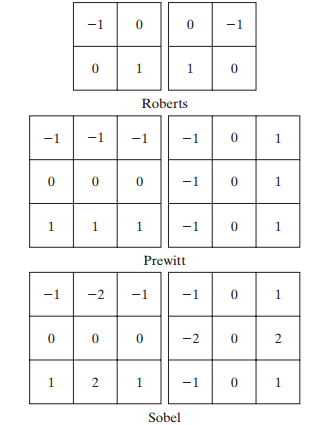
\includegraphics[scale=0.7]{myfigure/p9/3masks.png}
	\caption{3 masks for gradient computation: Roberts, Prewitt, Sobel}
	\label{fig:3masks}
\end{figure}

\subsubsection{More advanced techniques for edge detection}

